\documentclass[9pt]{extarticle}
\usepackage{graphicx} 
\usepackage{float}
\usepackage{booktabs}
\usepackage{array}
\usepackage{arydshln}
\usepackage{siunitx}
\usepackage{cancel}
\usepackage{changepage}
\usepackage{placeins}
\usepackage{siunitx}
\usepackage{lipsum}
\usepackage[most]{tcolorbox}
\usepackage{subcaption}
\usepackage{parskip}

\usepackage{times}
\usepackage{anyfontsize}
%\usepackage{mathpazo}
%\usepackage{tgtermes}

\usepackage{tabularx}
\usepackage{amsmath, amssymb, amscd, MnSymbol, mathrsfs}
\usepackage{cellspace}
\usepackage{tikz}
\usepackage{tikz-3dplot}
\usetikzlibrary{calc,3d, patterns, angles, quotes, decorations.markings, decorations.pathmorphing, hobby}
\usetikzlibrary{arrows.meta}
\usetikzlibrary{patterns.meta}
\tikzset{>=latex}
\usepackage{xfrac}
\usepackage{chemfig}
\usepackage{caption}
\usepackage{bm}
\usepackage{pdfpages}
\usepackage{pdflscape}
\usepackage{afterpage}
\usepackage{empheq}
\usepackage{pgfplots}
\usepackage{pgfplotstable}
\usepackage{xstring}
\pgfplotsset{compat=1.18}
\usepackage{textcomp}
\usetikzlibrary{external}
\tikzexternalize[prefix=figures/]

\usepackage{xcolor}


\usepackage{hyperref}
\usepackage{graphicx}
\usepackage{tabularray}
\usepackage{varwidth} 
\usepackage{mathtools}
\usepackage{scalerel}
%\usepackage{showframe}
\usepackage{fancyhdr}

\usepackage[left=0.8in,right=0.8in,top=0.5in,bottom=0.31in,includeheadfoot,letterpaper,footskip=0.02in]{geometry}
\pagestyle{fancy}
\fancypagestyle{plain}{
	\fancyhf{}
	\renewcommand{\headrulewidth}{0pt}
	\fancyhead[L]{\textit{S. Abiikar, F. Varley, A. Alireza et al.}}
	\fancyhead[R]{\textit{EG5016B - Exploring Engineering Project Management}}
	\fancyfoot[C]{\footnotesize\thepage}
}
\setlength{\headsep}{0.2in}


\usepackage{framed}
\newcommand{\formalsource}{}

\newenvironment{formal}[3][]{	\renewcommand{\formalsource}{#1}
	\def\lefty{\color{#2}\textquotedblleft}
	\def\righty{\color{#2}\textquotedblright}
	\def\FrameCommand{%
		\hspace{1pt}%
		{\color{#2}\vrule width 2pt}%
		{\color{#3}\vrule width 4pt}%
		\colorbox{#3}%
	}%
	\MakeFramed{\advance\hsize-\width\FrameRestore}%
	\begin{adjustwidth}{5pt}{7pt}%
		\ifx#2\empty\else\smash{\raisebox{-0.5em}{\Huge\lefty}}\hspace{0em}\fi%
	}{%
		\hspace{0em}\smash{\raisebox{-0.5em}{\Huge\righty}}\hfill%
		\ifx\formalsource\empty\else\hfill{\footnotesize\textit{\formalsource}}\fi%
	\end{adjustwidth}%
	\endMakeFramed%
	\noindent%
	\\
}

\newenvironment{formalt}[3][]{	
	\renewcommand{\formalsource}{#1}
	\def\lefty{\color{#2}\textquotedblleft}
	\def\righty{\color{#2}\textquotedblright}
	
	\def\FrameCommand{%
		\hspace{1pt}%
		{\color{#2}\vrule width 2pt}%
		{\color{#3}\vrule width 4pt}%
		\colorbox{#3}%
	}%
	
	\MakeFramed{\advance\hsize-\width\FrameRestore}%
\begin{adjustwidth}{-15pt}{0pt}%
	\ifx#2
	\empty
	\else
}{%
	\fi%
\end{adjustwidth}%
\vspace{0.5em}
\endMakeFramed%
	\noindent%
\\
}

\newcommand{\wm}[2]{%
	\begin{minipage}{#1\textwidth}
		#2
	\end{minipage}%
}


\usepackage{scalerel}

\usepackage[export]{adjustbox}
\usepackage{tocloft}
\renewcommand{\cfttoctitlefont}{}
\renewcommand{\contentsname}{}
\renewcommand{\cftsecleader}{\cftdotfill{\cftdotsep}}

\setlength{\cftbeforesecskip}{0.5em}



\usepackage{hyperref}    % For hyperlinks
\usepackage{xurl}        % better URL handling
\hypersetup{
	colorlinks=true,
	linkcolor=cyan!80!black,
	urlcolor=cyan!80!black,
	citecolor=cyan!80!black
}

\usepackage{caption}
\usepackage[export]{adjustbox}

\usepackage[para]{footmisc} % making footnotes run together in a paragraph


\usepackage{datetime}
\usepackage{datenumber}
\usepackage{etoolbox}

\usepackage{enumerate}
\usepackage{enumitem}

\usepackage{ifthen}
\usepackage{calc}
\usepackage{physics}
\usepackage{shapepar,transparent}


% ====== DEADLINE SETUP ======
\newcounter{deadlineyear}\setcounter{deadlineyear}{2025}
\newcounter{deadlinemonth}\setcounter{deadlinemonth}{12} % December
\newcounter{deadlineday}\setcounter{deadlineday}{15}
\newcounter{deadlinetime}\setcounter{deadlinetime}{0} % Will be set via macro

% ====== OTHER COUNTERS ======
\newcounter{mydatenumber}
\newcounter{currentdate}
\newcounter{daysdiff}
\newcounter{currenttime}
\newcounter{totalminutes}
\newcounter{displaydays}
\newcounter{remainingmins}
\newcounter{displayhours}
\newcounter{displaymins}

% ====== MACROS ======
% Set deadline time (HH, MM)
\newcommand{\setdeadlinetime}[2]{%
	\setcounter{deadlinetime}{\numexpr #1*60 + #2\relax}%
}

% ====== MAIN COMMAND ======
\newcommand{\timeUntilDeadline}{%
	% Calculate date difference
	\setmydatenumber{mydatenumber}{\value{deadlineyear}}{\value{deadlinemonth}}{\value{deadlineday}}%
	\setmydatenumber{currentdate}{\year}{\month}{\day}%
	\setcounter{daysdiff}{\numexpr\value{mydatenumber} - \value{currentdate}\relax}%
	% Current time (in minutes since midnight)
	\setcounter{currenttime}{\time}%
	% Total minutes until deadline
	\setcounter{totalminutes}{\numexpr\value{daysdiff}*1440 + \value{deadlinetime} - \value{currenttime}\relax}%
	% Display result
	\ifnum\value{totalminutes}<0
	\textbf{\color{red}Deadline passed!}%
	\else
	% Breakdown
	\setcounter{displaydays}{\numexpr\value{totalminutes}/1440\relax}%
	\setcounter{remainingmins}{\numexpr\value{totalminutes}-\value{displaydays}*1440\relax}%
	\setcounter{displayhours}{\numexpr\value{remainingmins}/60\relax}%
	\setcounter{displaymins}{\numexpr\value{remainingmins}-\value{displayhours}*60\relax}%
	% Output
	{%
		\ifnum\value{displaydays}>0
		\thedisplaydays\ day\ifnum\value{displaydays}>1 s\fi%
		\ifnum\value{displayhours}>0\ and \fi%
		\fi%
		\ifnum\value{displayhours}>0
		\thedisplayhours\ hour\ifnum\value{displayhours}>1 s\fi%
		\ifnum\value{displaymins}>0\ and \fi%
		\fi%
		\ifnum\value{displaymins}>0
		\thedisplaymins\ minute\ifnum\value{displaymins}>1 s\fi%
		\fi
		}%
	\fi
}


\usepackage{titlesec}


%\renewcommand{\thechapter}{\bfseries\Alph{chapter}} 
%\renewcommand{\chaptername}{\bfseries Part} 

\titleformat{\chapter}[block]{\Huge\raggedright}{\chaptername\;\thechapter\\[0.5em]}{0pt}{\Huge\raggedright}

\renewcommand{\thesection}{\arabic{section}.}
\renewcommand{\thesubsection}{\thesection\arabic{subsection}}
\renewcommand{\thesubsubsection}{\thesubsection.\arabic{subsubsection}}

\titleformat{\section}[block]{\large\bfseries\raggedright}{\thesection}{0.5em}{}
\titleformat{\subsection}[block]{\raggedright}{\thesubsection}{0.5em}{}
\titleformat{\subsubsection}[block]{\raggedright}{\thesubsubsection}{0.5em}{}



\def\customhrule{\hrule\vspace{1em}\noindent}

%\usepackage{darkmode}
%\enabledarkmode


\begin{document}
\tikzexternaldisable

	\thispagestyle{empty}
	\centering
	\Huge
	Conceptual frame for a large-scale electrolyser vessel\\[0.8em]
	\normalsize %\textit{Application for aiding vertical motion}\\	
\large
Sakariye Abiikar$^{\hyperlink{affilA}{\text{a}},\hyperlink{corresp}{\dagger}}$%
\begingroup
\renewcommand
\thefootnote{}\footnotetext{%
	\hypertarget{corresp}{}% target for dagger
	\textsuperscript{\footnotesize\dagger}\kern0.3em Corresponding author.\\
	\wm{0.6}{\vspace{0.5em}\hspace{1.6em}\textit{E-mail address:} \;\href{mailto:k2371673@kingston.ac.uk}{k2371673@kingston.ac.uk} (S. Abiikar).}
} 
\addtocounter{footnote}{-1}
\endgroup
\kern-0.4em, Freddie Varley$^{\hyperlink{affilA}{\text{a}}}$, 
Alishahi Alireza$^{\hyperlink{affilA}{\text{a}}}$, 
Ihsan Muhammad Humayon$^{\hyperlink{affilA}{\text{a}}}$, \\
Sangireddy Vrishin R$^{\hyperlink{affilA}{\text{a}}}$ \\[0.4em]
\small
\hypertarget{affilA}{\textsuperscript{a}\,\textit{Department of Mechanical Engineering, Kingston University, London, UK}}\\[0.6em]
	\footnotesize
	Deadline: Monday 15$^{\text{th}}$ December, 2025 [23:59], Last Updated: \today \,[\currenttime],\\ Days left until deadline: \timeUntilDeadline.\\
	\normalsize
	\raggedright
	\vspace{3em}
	\hrule	\vspace{-0.1em}
\section*{Abstract}\vspace{-0.4em}
\hspace{1em}This report presents the \textit{development} of an {assembly and maintenance frame} for Supercritical Solutions' large-scale electrolyser vessel. The project uses the {DMAIC framework} to guide systematic problem definition, measurement, analysis, improvement, and control. Design concepts are generated, evaluated, and optimized to satisfy technical, operational, and sustainability requirements, while integrating stakeholder and customer needs through tools such as the {Voice of the Customer (VoC)} and {Objective Tree Diagram (OTD)}. Risk management, including {DFMEA}, and quality control measures are applied to ensure a robust, safe, and practical solution. The report documents methodology, key design decisions, and professional competencies developed.\\[2em]
\hrule
\section{Introduction}
Electrolysers play a critical role in industrial hydrogen production, requiring {robust support structures} for safe and efficient operation. Designing assembly and maintenance frames for large-scale vessels presents challenges including structural integrity, accessibility, maintenance, and long-term reliability.\\[0.8em]
This project focuses on developing an assembly and maintenance frame for Supercritical Solutions’ electrolyser vessel, applying {systems thinking} and the {DMAIC methodology}. Stakeholder and customer requirements are captured using {VoC} and {OTD}, while design evaluation uses tools such as {QFD} and concept trade-off analysis. Risk assessment via {DFMEA} and quality planning ensure compliance with technical, operational, and sustainability standards.\\[0.8em]
The report outlines project methodology, key engineering decisions, and rationale behind the chosen solution, highlighting professional skills developed including {project management}, {teamwork}, {critical thinking}, and {problem-solving}.

%\begin{itemize}[itemsep=-1mm]
%	\item \textbf{Customer and Stakeholder Requirements}: List functional requirements (load support, accessibility, safety, ergonomics) using \textbf{VoC}.
%	\item \textbf{Project Objectives}: Include \textbf{OTD} showing link from high-level goals to design targets.
%	\item \textbf{Constraints and Specifications}: Material, dimensional, regulatory, cost, and sustainability requirements.
%\end{itemize}

\section{Define (D)}
\begin{minipage}[t]{0.5\textwidth}\vspace{-1.2em}\hspace{-1em}
	\tikzexternalenable
	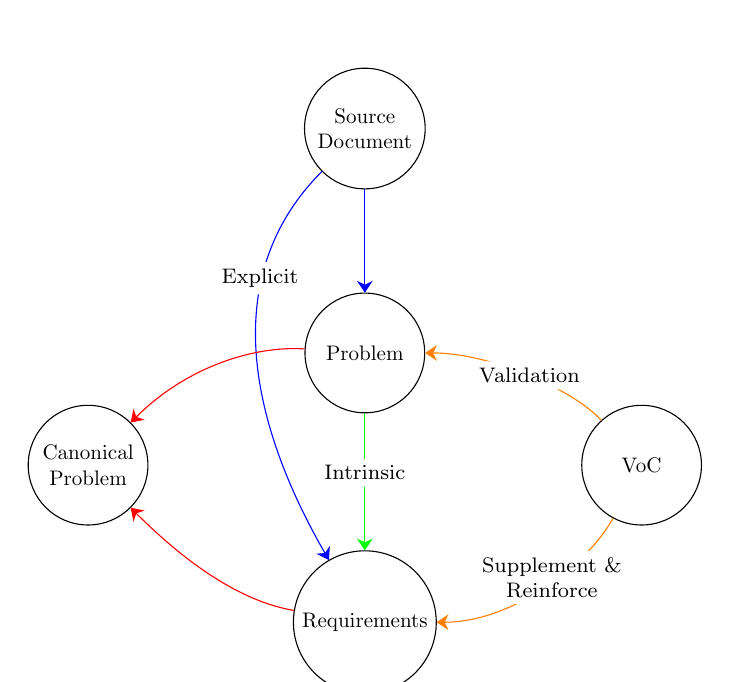
\begin{tikzpicture}[
		scale=0.95,
		every node/.append style={transform shape},    
		myarrow/.style={-{Stealth[length=1.5mm,width=2mm]}}]
		\node[draw, circle, minimum size=2cm, align=center, scale=0.8] (source) at (0,0) {Source\\Document};
		\node[draw, circle, minimum size=2cm, align=center, scale=0.8] (problem) at (0,-3) {Problem};
		\node[draw, circle, minimum size=2cm, align=center, scale=0.8] (req) at (0,-6.6) {Requirements};
		\node[draw, circle, minimum size=2cm, align=center, scale=0.8] (final) at (-3.7,-4.5) {Canonical\\Problem};
		\node[draw, circle, minimum size=2cm, align=center, scale=0.8] (voc) at (3.7,-4.5) {VoC};
		\draw[myarrow,blue] (source) -- (problem);
		\draw[myarrow,green] (problem) -- (req);
		\node[fill=white, draw=white, line width=3pt, inner sep=1pt, rounded corners=2pt, font=\footnotesize] at (0,-4.6) {Intrinsic};
		\draw[myarrow,blue] (source) .. controls (-2,-2) and (-1.5,-4) .. (req);
		\node[fill=white, draw=white, line width=3pt, inner sep=1pt, rounded corners=2pt, font=\footnotesize,xshift=17pt] at (-2,-2) {Explicit};
		\draw[myarrow,red] (problem) .. controls (-1.5,-2.9) and (-2.4,-3.2) .. (final);
		\draw[myarrow,red] (req) .. controls (-1.8,-6.3) and (-2.6,-5.6) .. (final);
		\draw[myarrow,orange] (voc) .. controls (2.8,-3.5) and (1.7,-3) .. (problem);
		\node[fill=white, draw=white, line width=3pt, inner sep=1pt, rounded corners=2pt, font=\footnotesize] at (2.2,-3.3) {Validation};
		\draw[myarrow,orange] (voc) .. controls (3,-5.8) and (2,-6.6) .. (req);
		\node[fill=white, draw=white, line width=3pt, inner sep=1pt,
		rounded corners=2pt, font=\footnotesize, align=center]
		at (2.5,-6) {Supplement \&\\Reinforce};
	\end{tikzpicture}\\
	\tikzexternaldisable
	\begin{minipage}{0.9\linewidth}
		\vspace{2em}
		\captionof{figure}{\centering Define Phase Workflow\\ From Source to Canonical Problem}
	\end{minipage}
\end{minipage}\hfill
\begin{minipage}[t]{0.5\textwidth}
	\vspace*{-1em}
	\subsection{Approach Overview}
	This Define phase establishes a clear and validated understanding of the problem by consolidating information from the Initial Industry Brief, Voice of the Customer (VoC), and stakeholder inputs. Our approach follows a structured path:\\[-0.3em]
	\begin{itemize}[itemsep=2mm]
		\item Extract key information from the Industry Live Brief to identify preliminary problems.
		\item Validate and refine these problems and requirements through VoC feedback.
		\item Translate validated insights into measurable requirements and objectives.
		\item Define material, dimensional, and regulatory constraints to ground the design in feasibility.
	\end{itemize}\vspace{1.2em}
By integrating information from source documents, VoC feedback, and iterative analysis, the problem definition is anchored in reality and precisely specified.\\[0.8em]
This combination of context, explicit formulation, and validation produces a well-defined problem statement that clearly identifies requirements, objectives, and constraints, establishing a solid foundation for subsequent concept development and evaluation.
\end{minipage}

\newpage

\thispagestyle{plain}
\subsection{Industry Live Brief Breakdown}
\begin{minipage}{0.58\textwidth}
Our initial source document is the live brief provided by {Supercritical Solutions Ltd}, which defines the project title as:\\[-0.6em]
\begin{formal}[Zaarour, 2025, p. 1]{black}{white}
\textit{	Designing an assembly and maintenance frame for Supercritical’s large-scale electrolyser vessel.}
\end{formal}\\[-1.8em]
The title establishes the project’s core intent to \textbf{design} a frame for assembly and maintenance of a critical industrial component; The synopsis of the brief begins as follows:\\[-0.6em]
\begin{formal}[Zaarour, 2025, p. 1]{black}{white}
\textit{	This project focuses on developing a conceptual assembly and maintenance frame for a large-scale electrolyser module. The outer vessel houses several internal sub-units (“black boxes”), designed for efficient replacement, inspection, and servicing.}
\end{formal}\\[-1.8em]
This highlights the project’s \textbf{conceptual} phase, emphasizing design intent over production. It introduces a vessel-based system containing modular internal units, indicating that serviceability, accessibility, and efficient replacement are key design priorities.\\[1em]
\end{minipage}\hfill
\begin{minipage}{0.4\textwidth}
    \includegraphics[width=0.85\linewidth, trim=10pt 5pt 10pt 5pt, clip]{../../../Pictures/Screenshots/swappy-20251019-211642}
    \captionof{figure}{Zaarour, 2025, p.1,2}
\end{minipage}\\\vspace{-0.6em}
\begin{formal}[Zaarour, 2025, p. 1]{black}{white}
\textit{	At a high level, the process involves securing the vessel, lifting and positioning the internal units, and enabling disassembly without compromising safety, alignment, or component integrity. A conceptual frame will be proposed to support this process.}
\end{formal}
Here, the operational workflow is defined. The frame must perform under heavy loads, maintain precise alignment, and allow repeatable assembly and disassembly. This introduces key engineering considerations such as load path design, lifting safety, and tolerance management. It also frames the system as one that supports {both assembly and maintenance}, implying a dual-purpose design philosophy.\\[1em]
\begin{formal}[Zaarour, 2025, p. 1]{black}{white}
\textit{	The frame design prioritises {ergonomics}, ensuring operators can safely access and manipulate heavy components while reducing manual strain. Safety features, such as interlocks and shielding, will mitigate risks during lifting and positioning. Automation elements—like guided lifting systems or robotic assistance—will improve repeatability, reduce error, and shorten turnaround time during both assembly and maintenance cycles.}
\end{formal}
This passage adds a human and process-oriented layer. The focus shifts from mechanical function to {operator safety, efficiency, and automation}. \textbf{Ergonomics} becomes a measurable design driver, suggesting the integration of human factors engineering. Automation hints at the use of advanced control systems or assistive mechanisms, raising new requirements for precision, reliability, and system integration.

\begin{formal}[Zaarour, 2025, p. 2]{black}{white}
\textit{	The project plan will include mapping of assembly/disassembly workflows, conceptual frame design, and an evaluation of tooling requirements. Risks to address include component misalignment, equipment handling hazards, and delays from non-standardised interfaces. Quality considerations will centre on ensuring precision fits, traceability of maintenance activities, and robustness of the rig to repeated use.}
\end{formal}
This formalises the project management expectations. It highlights risk-based thinking and introduces the need for workflow mapping — key aspects of the DMAIC and systems engineering approaches. The emphasis on quality, traceability, and standardisation implies that the solution must not only perform mechanically but also fit within broader operational and maintenance systems.\\[1em]
%\item The solution must be \textbf{modular and reusable}, not a single-use fixture.
\begin{formal}[Zaarour, 2025, p. 2]{black}{white}
\textit{	The outer vessel measures 870 mm internal diameter × 3000 mm internal height (1100 mm OD × 3500 mm total height) and weighs 13 tons. Housed within the vessel are internal sub-units, collectively forming a “black box” assembly measuring 550 × 550 × 2000 mm in height, with a combined weight of 3 tons. These sub-units are attached to the vessel lid, and must be safely lifted, positioned, and removed during assembly and maintenance cycles.}
\end{formal}
The scale of the engineering problem is defined by the physical constraints of the system. The vessel's significant height (~3m) and limited internal clearance are compounded by the sizable sub-units (2000mm, 3 tons) attached to the lid. This configuration presents a critical handling challenge: ensuring the precise, sway-free vertical translation of the sub-units to avoid contact with the vessel walls. With interaction limited solely to the lid, the problem is one of extreme spatial restriction. The following client questions (VoC) have been id	entified:
\begin{formalt}[]{blue}{blue!5!white}
\begin{quote}
	"Can we assume that no modifications or attachments are allowed on the vessel or the internal components?\\[0.2em]
	\small\hspace{4em}- If not (we are allowed), are there preferred methods or restrictions for supporting the sub-units from the lid?\\ \normalsize and are there any additional operational constraints that haven't been outlined?"
\end{quote}
\end{formalt}
	
\begin{formal}[Zaarour, 2025, p. 2]{black}{white}
\textit{Consider vertical vs horizontal assembly/maintenance option. 
\begin{itemize}[itemsep=-1mm]
	\item \textbf{Vertical assembly:} Relies on sufficient clearance and workshop ceiling heights.
	\item \textbf{Horizontal assembly:} Involves assembling internal sub-units on a cradle or skid, using restraints to safely move the parts into the vessel and provide stability during the rotation operation to reach the final vertical assembly.
\end{itemize}}
\end{formal}
The use of the term \textbf{consider} indicates that the brief leaves the choice of assembly orientation open.
If vertical assembly is chosen, it remains unclear what the maximum allowable ceiling height and workspace constraints are, yes that is true, but by logic, the ceiling must be at least: 

\begin{enumerate}[label=\arabic*)]
	\item The height of the vessel itself.
	\item Plus the height of the internal sub-units attached to the vessel lid so that it would be about to be taken out.
\end{enumerate}

Both conditions must be satisfied for vertical assembly to be feasible, so the frame would be built around those being true.  

For horizontal assembly, questions arise regarding the method for stabilizing the sub-units during rotation, acceptable tolerances for positioning, and whether specific tools or fixtures are required. For this scenario to be viable, the “black box” components would need to be supported to prevent sagging for the chance that it exists since the horizontal nature introduces this, however, if the components are held inside the vessel for stabilization, the steps for removal and insertion become unclear, making the workflow and visualization of the assembly process more ambiguous.\\[0.7em]
These observations prompt questions for the client such as: 
\begin{formalt}[]{blue}{blue!5!white}
	\begin{quote}
		“Do we select a single assembly orientation and neglect the other, or must both be accommodated? Are the mechanisms for vertical and horizontal assembly interchangeable, or do they require separate designs? How does this choice influence prioritisation and design approach?”
	\end{quote}
\end{formalt}
Areas where direct input from the client would clarify design requirements, reduce ambiguity, and ensure that the chosen approach is feasible and well-defined.
\subsection{OTD}

\newpage

\subsection{Summary and Interpretations (Draft)}
%The live brief defines the project’s conceptual aim: designing a frame to enable assembly and maintenance of a large-scale electrolyser vessel and its internal sub-units. From this, the core engineering problem can be interpreted as creating a physical system that allows safe, repeatable handling of the internal modules without compromising alignment, safety, or component integrity.  
%
%\textbf{Key Project Requirements:}
%\begin{itemize}[itemsep=-1mm]
%	\item \textbf{Vessel support:} Stabilize the vessel (870 mm ID × 3000 mm height, 13 tons) while allowing safe access.
%	\item \textbf{Sub-unit handling:} Lift, position, and remove internal “black box” modules (550 × 550 × 2000 mm, 3 tons) with precision.
%	\item \textbf{Operator access and ergonomics:} Ensure safe manipulation of heavy components.
%	\item \textbf{Alignment and repeatability:} Maintain precise positioning during insertion/removal.
%	\item \textbf{Safety features:} Protect against collisions or accidents during handling.
%	\item \textbf{Workflow integration:} Support standardized assembly and maintenance procedures.
%\end{itemize}
%
%This interpretation frames the system as a \textbf{dual-purpose assembly and maintenance frame}, guiding the creation of: 
%
%\begin{itemize}[itemsep=-1mm]
%	\item Preliminary conceptual layouts showing the frame’s interaction with the vessel and sub-units.
%	\item Tables of inputs (weights, dimensions, forces, operator interactions) and outputs (movement paths, supported loads, safety clearances, workflow steps).
%	\item Identification of key mechanical, ergonomic, and operational constraints for the early design stage.
%\end{itemize}





\newpage

\section{Measure (M)}
\color{red!50!black}
\begin{itemize}[itemsep=-1mm]
	\item \textbf{Existing System Analysis}: Identify limitations in current supports/frames.
	\item \textbf{Structural and Operational Data}: Vessel dimensions, weight, centre of mass, lifting points.
	\item \textbf{SWOT Analysis}: Strengths, weaknesses, opportunities, and threats of current design.
\end{itemize}
\color{black}
\newpage

\section{Analyse (A)}
\color{red!50!black}
\begin{itemize}[itemsep=-1mm]
	\item \textbf{Concept Generation}: Brainstorm frame geometries, assembly approaches, and maintenance access strategies.
	\item \textbf{Concept Selection}: Use \textbf{Pugh Matrix} and evaluate trade-offs (cost vs. performance vs. safety).
	\item \textbf{Risk Assessment}: DFMEA of potential failure modes in assembly, lifting, and operation.
	\item \textbf{Design Calculations}: Structural analysis (stress, deflection, factor of safety), material selection.
\end{itemize}
\color{black}
\newpage

\section{Improve (I)}
\color{red!50!black}
\begin{itemize}[itemsep=-1mm]
	\item \textbf{Final Design Concept}: Detailed drawings, CAD models, and key dimensions.
	\item \textbf{Optimization}: Geometry adjustments for weight reduction, improved access, cost efficiency.
	\item \textbf{Quality Control Measures}: Checkpoints for fabrication and assembly; integration of PDCA cycle.
\end{itemize}
\color{black}

\newpage

\section{Control (C)}
\color{red!50!black}
\begin{itemize}[itemsep=-1mm]
	\item \textbf{Implementation Plan}: Stepwise assembly and maintenance protocols.
	\item \textbf{Final Risk Mitigation}: Address critical DFMEA items.
	\item \textbf{Sustainability and Lifecycle}: Material recyclability, maintenance requirements, durability.
	\item \textbf{Verification}: Ensure design meets technical, operational, and stakeholder requirements.
\end{itemize}
\color{black}

\newpage

\section{Conclusion}
\color{red!50!black}
Summarize how the frame meets functional, safety, and sustainability goals. Highlight trade-offs, engineering analysis applied, and design optimization. Reflect on professional skills developed: problem-solving, teamwork, and project management.
\color{black}

\newpage

\section{Appendices}
\color{red!50!black}
\begin{itemize}[itemsep=-1mm]
	\item Supporting calculations, sketches, CAD screenshots.
	\item DFMEA table.
	\item OTD and QFD diagrams.
	\item Meeting minutes and stakeholder feedback.
\end{itemize}
\color{black}

%\newpage\pagenumbering{gobble}
%\chapter{Project Scope and Goals}
%\newpage\pagenumbering{arabic}\setcounter{page}{1}

\newpage

\subsection*{Reference}
Zaarour, A. (2025). \textit{Industry Live Brief: Designing an assembly and maintenance frame for Supercritical's large-scale electrolyser vessel} [PDF]. EG5016B – Exploring Engineering Project Management. Kingston University London.

\url{https://knowledgebase.nexpcb.com/articles/assembly-types-and-levels/}
\url{https://en.wikipedia.org/wiki/Maintenance}

\end{document}


\newpage\pagenumbering{gobble}
\chapter{Design Development}
\newpage\pagenumbering{arabic}\setcounter{page}{\numexpr\thepage+1}

empty

\newpage\pagenumbering{gobble}
\chapter{Finalized Design}
\newpage\pagenumbering{arabic}\setcounter{page}{\numexpr\thepage+1}

\section{Main Concept Overview}
\subsection{Concept Summary}
Present a clear, concise description of your final design concept, outlining its primary function, key innovation, and intended user benefit.

\subsection{Reverse Engineering Pathway}
Include a visual flowchart showing the systematic development process. Clearly map how each tool (VoC, OTD, HoQ) contributed to specific design decisions and the final concept.

\section{Voice of the Customer (VoC)}
\subsection{Insights from Questionnaire}
Present 3-4 key insights derived from customer questionnaire responses that directly shaped your understanding of customer needs.

\subsection{Summary of Needs}
Briefly summarise the primary customer needs identified from the VoC analysis that directly influenced your design concept.

\section{Objective Tree Diagram (OTD)}
\subsection{Key Objectives}
Display 3-4 main objectives from your OTD that guided the design development.

\subsection{Visual Representation}
Include a simplified version of your OTD showing how these objectives link hierarchically to your final concept.

\section{House of Quality (HoQ)}
\subsection{Highlighted Requirements}
Present 3 key customer requirements and 5 corresponding functional requirements that were most critical in shaping your design.

\subsection{Design Integration}
Explain how each highlighted requirement influenced specific aspects of your final design concept.\\
\newpage

\section{Systems Engineering Integration}
\subsection{Holistic Approach}
Describe how you applied Systems Engineering principles to ensure all project elements worked together as a cohesive system.

\subsection{Customer and Stakeholder Needs}
Explain how Systems Engineering helped you address both customer and stakeholder needs throughout the design process.

\subsection{Interdependencies}
Briefly discuss how you considered and managed interdependencies between different components of your concept.

\section{Design for X (DfX)}
\subsection{Factor Focus Area}
Select and state one DfX factor (e.g., Design for Manufacturability or Sustainability) that significantly impacted your design.

\subsection{Explanation}
Describe how this DfX factor influenced specific design choices to enhance functionality, manufacturability, or sustainability.

\section{Hypothesised Failures (DFMEA)}
\subsection{Potential Failures}
Identify 1-2 main failure modes anticipated in your DFMEA analysis.

\subsection{Preventative Actions}
Summarise the specific mitigations implemented in your design to address these potential failures.


	\newpage
	
	
%	\newpage\pagenumbering{gobble}
%	\noindent	
%	\huge Table of Contents\\
%	\normalsize
%	{
%		\hypersetup{linkcolor=black}
%		\tableofcontents
%	}    	
%	\thispagestyle{empty}
%	{
%		\hypersetup{linkcolor=black}
%		\pagenumbering{gobble}
%		\tableofcontents
%	}    
%	\newpage\newgeometry{left=0.8in,right=0.8in,top=1in,bottom=0.3in}
%	\noindent\pagenumbering{arabic}\setcounter{page}{1}


	
	



	
\end{document}
